%%%%%%%%%%%%%%%%%%%%%%%%%%%%%%%%%%%%%%%%%%%%%%%%%%%%%%%%%%%%%%%%%%%%%%%%%%
%%LaTeX template for papers && theses									%%
%%Done by the incredible ||Z01db3rg||									%%
%%Under the do what ever you want license								%%
%%%%%%%%%%%%%%%%%%%%%%%%%%%%%%%%%%%%%%%%%%%%%%%%%%%%%%%%%%%%%%%%%%%%%%%%%% 

%start preamble
\documentclass[paper=a4,fontsize=11pt]{scrartcl}%kind of doc, font size, paper size
\usepackage[ngerman]{babel}%for special german letters etc			
%\usepackage{t1enc} obsolete, but some day we go back in time and could use this again
\usepackage[T1]{fontenc}%same as t1enc but better						
\usepackage[utf8]{inputenc}%utf-8 encoding, other systems could use others encoding
%\usepackage[latin9]{inputenc}			
\usepackage{amsmath}%get math done
\usepackage{amsthm}%get theorems and proofs done
\usepackage{graphicx}%get pictures & graphics done
\graphicspath{{pictures/}}%folder to stash all kind of pictures etc
\usepackage[pdftex,hidelinks]{hyperref}%for links to web
\usepackage{amssymb}%symbolics for math
\usepackage{amsfonts}%extra fonts
\usepackage []{natbib}%citation style
\usepackage{caption}%captions under everything
\usepackage{listings}
\usepackage[titletoc]{appendix}
\numberwithin{equation}{section} 
\usepackage[printonlyused,withpage]{acronym}%how to handle acronyms
\usepackage{float}%for garphics and how to let them floating around in the doc
\usepackage{cclicenses}%license!
\usepackage{xcolor}%nicer colors, here used for links
\usepackage{wrapfig}%making graphics floated by text and not done by minipage
\usepackage{dsfont}
\usepackage{stmaryrd}
\usepackage{geometry}
\usepackage{hyperref}
\usepackage{fancyhdr}
\usepackage{menukeys}

\pagestyle{fancy}
\lhead{Benjamin Tröster\\Netzwerke Seminaristische Übung (WS17/18)}
\rhead{
\includegraphics[scale=0.5]{htw2}}
\lfoot{Übungsblatt 5 -- IP \& Routing Teil 2}
\cfoot{}
\fancyfoot[R]{\thepage}
\renewcommand{\headrulewidth}{0.4pt}
\renewcommand{\footrulewidth}{0.4pt}

\lstdefinestyle{Bash}{
  language=bash,
  showstringspaces=false,
  basicstyle=\small\sffamily,
  numbers=left,
  numberstyle=\tiny,
  numbersep=5pt,
  frame=trlb,
  columns=fullflexible,
  backgroundcolor=\color{gray!20},
  linewidth=0.9\linewidth,
  %xleftmargin=0.5\linewidth
}


\newlength\labelwd
\settowidth\labelwd{\bfseries viii.)}
\usepackage{tasks}
\settasks{counter-format =tsk[a].), label-format=\bfseries, label-offset=3em, label-align=right, label-width
=\labelwd, before-skip =\smallskipamount, after-item-skip=0pt}
\usepackage[inline]{enumitem}
\setlist[enumerate]{% (
labelindent = 0pt, leftmargin=*, itemsep=12pt, label={\textbf{\arabic*.)}}}

\pdfpkresolution=2400%higher resolution

%settings colors for links
%\hypersetup{
 %   colorlinks,
  %  linkcolor={blue!50!black},
   % citecolor={blue},
    %urlcolor={blue!80!black}
%}

%\usepackage[pagetracker=true]{biblatex}

%%here begins the actual document%%
\newcommand{\horrule}[1]{\rule{\linewidth}{#1}} % Create horizontal rule command with 1 argument of height

\begin{document}
\begin{center}
~\\
\Large{\textbf{Übungsblatt 5 -- OSI Network Layer}}
\end{center}
\large{\textbf{\textcolor{red}{Hinweis:} Versuchen Sie die Übungsblätter soweit wie möglich ohne Hilfe von Google, Stackoverflow, Stackexchange zu lösen. Sie sollen eigene Lösungswege finden und nicht professionell Suchmaschinen bedien können. Ausnahmen sind natürlich Aufgaben, in denen explizit recherchiert werden soll}

\begin{center}\Large{\textbf{Aufgabe A -- Einrichten eines komplexen Netzwerkes mithilfe von Linux-Routern}}\end{center}\vskip0.25in
Wir erweitern nun das vorhandene Netzwerk dergestalt, dass ein weiterer Rechner aus
jeder Reihe zum Router umgebaut wird. Wenn genug Raspberry Pis vorhanden sind, kann auch ein zusätzlicher Raspberry Pi an den Switch angeschlossen werden. Der neue Router soll alle Pakete, die an Rechner außerhalb des eigenen Netzes gerichtet sind, in die anderen Reihen weiterleiten können. Somit können Sie dann jeden beliebigen Raspberry Pi im Labor \glqq anpingen\grqq. Die Router sorgen dafür, dass alle Pakete über den \glqq Backbone\grqq\ zu Ihrem Ziel geleitet werden. Im wesentlichen soll das Netzwerk wie in Abbildung \ref{backbone} umgesetzt werden. 
\begin{figure}[H]
	\center
	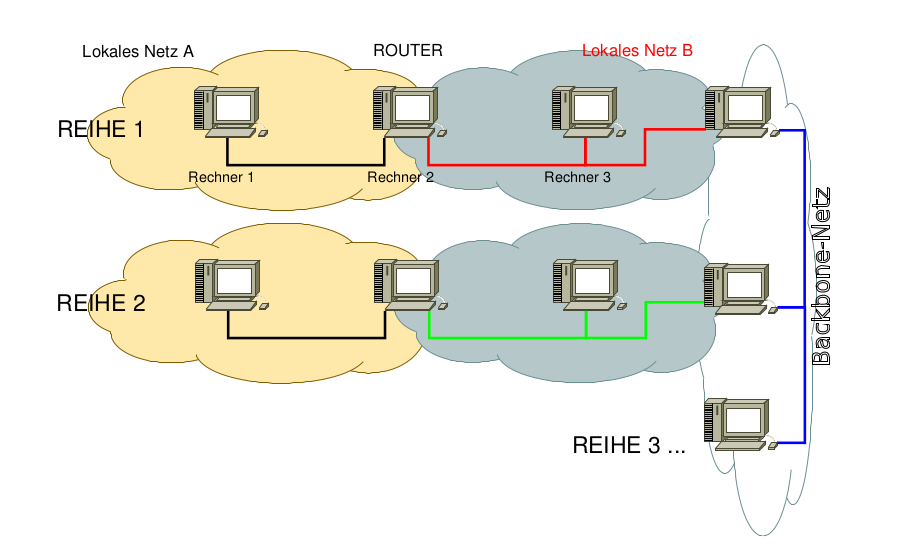
\includegraphics[scale=0.4]{backbone}
	\caption{Backbone-Netzwerk}
	\label{backbone}
\end{figure}
\vskip0.05in ~\\
\textbf{Achtung:} Da es in dem Backbone-Netz fünf gleichwertige Router gibt, können Sie hier nicht mit \glqq Default-Routes\grqq\ arbeiten! Sie müssen auf den Backbone-Rechnern nun mehrere explizite Routen mit einem Zielnetzwerk und zugehöriger Subnetzmaske eintragen.
\begin{tasks}(1)
	\task Wählen Sie einen Rechner aus Ihrer Reihe der noch nicht als Router fungiert. Geben Sie diesem Router eine zweite IP-Adresse 172.32.250.X, wobei $X =$ Nummer Ihrer Reihe entspricht.
	\task Aktivieren Sie hier auch wieder das Routing und tragen Sie alle Routen zu den anderen Reihen ein.
	\task Prüfen Sie mit \emph{ping} ob Sie alle Rechner erreichen können -- bei welchen Rechner klappt es und bei welchen nicht?
	\task Was müssen Sie jetzt noch an der Konfiguration einer oder aller anderen Rechner Ihrer Reihe anpassen, damit sich wirklich alle Rechner anpingen können (bzw. als Teilschritt davor -- alle können den Backbone-Router anpingen).
	\task Prüfen Sie mit \emph{ping} ob Sie jetzt wirklich alle Rechner erreichen können.
	\task Prüfen Sie mit Wireshark auf dem neuen Backbone-Router, ob auch alle Pakete wirklich über diesen Rechner geleitet werden oder vielleicht irgendein Rechner eine \glqq Abkürzung\grqq\ nimmt.
\end{tasks}
\begin{center}\Large{\textbf{Aufgabe B -- Einrichtung des Uplinks}}\end{center}\vskip0.25in
Seitdem wir den DHCP-Dienst auf den Raspberry Pis ausgeschaltet haben, haben wir keinen Uplink ins Internet mehr. Das soll sich mit dieser Aufgaben ändern.\\
Um den Raspberry Pis eine Möglichkeit zu geben sich mit dem Internet zu verbinden, soll ein Uplink eingerichtet werden. Das heißt: Ihr konfigurierter Router soll dafür sorgen, dass sie beispielsweise die Webseite der HTW-Berlin anpingen können.
\begin{tasks}
  \task Erweitern Sie den Router, sodass dieser den Uplink im Labor nutzen kann. Der Uplink ist auf dem Server im Dell-Rack untergebracht und besitzt die IP-Adresse: 10.10.10.254. Wie Sie bereits vermuten werden, muss Ihr Router nun die Pakete in dieses Netz bzw. an diesen Server weiterleiten können. Konfigurieren Sie entsprechend Ihren Router zunächst mit den Ihnen bekannten Tools \glqq on the fly \grqq.
  \task Wenn Ihre Lösung funktioniert: Nehmen Sie eine persistente Umsetzung vor, die einen Reboot übersteht. 
  \task Um nicht nur IP-basiert anfragen stellen zu können (aber auch um bspw. Updates erhalten zu können) muss der Router eine Namensauflösung vornehmen können. Hierfür ist ein sogenannter DNS-Server ebenfalls auf dem Uplink eingerichtet. Recherchieren Sie kurz, was die Aufgaben eines DNS-Servers sind und wie im groben eine Namensauflösung vonstatten geht.
  \task Die Namensserver werden unter Debian-Linux in der \emph{resolv.conf} abgelegt, in dieser Datei können die IP-Adressen der DNS-Server eingetragen werden, die zur Namensauflösung befragt werden sollen. Für die Umsetzung der Namensauflösung soll nun die IP-Adresse des Uplinks eingetragen werden.
  \task Nachdem Sie den Namensserver eingetragen und der Router konfiguriert wurde, sollen Sie nun die Adresse \emph{htw-berlin.de} anpingen.
\end{tasks}
\end{document}